\chapter{\label{method}Description of CLD detectors$^{\cite{CLD}}$}

\setcounter{equation}{0}
\setcounter{table}{0}
\setcounter{figure}{0}

\baselineskip 20pt
\hspace{10pt}
\section{Dimension and layout}
In this following sections we have described the  possible future  CLD detector for 
FCC-ee \cite{CLD}. This detector  have  a silicon 
pixel vertex detector and a silicon tracker, followed by highly 
granular calorimeters (a silicon-tungsten ECAL and a 
scintillator-steel
HCAL). A superconducting solenoid provides a strong magnetic 
field, and a steel yoke interleaved with
resistive plate (RPC) muon chambers closes the magnetic field.
At this stage of the design of detector, it is assumed that the detector is identical for all the collision energies of FCC-ee, i.e. for operation at the $Z (91.2 GeV)$, $W (160 GeV)$, $H (240 GeV)$ and $top (365 GeV)$.
\begin{figure}
    \centering
    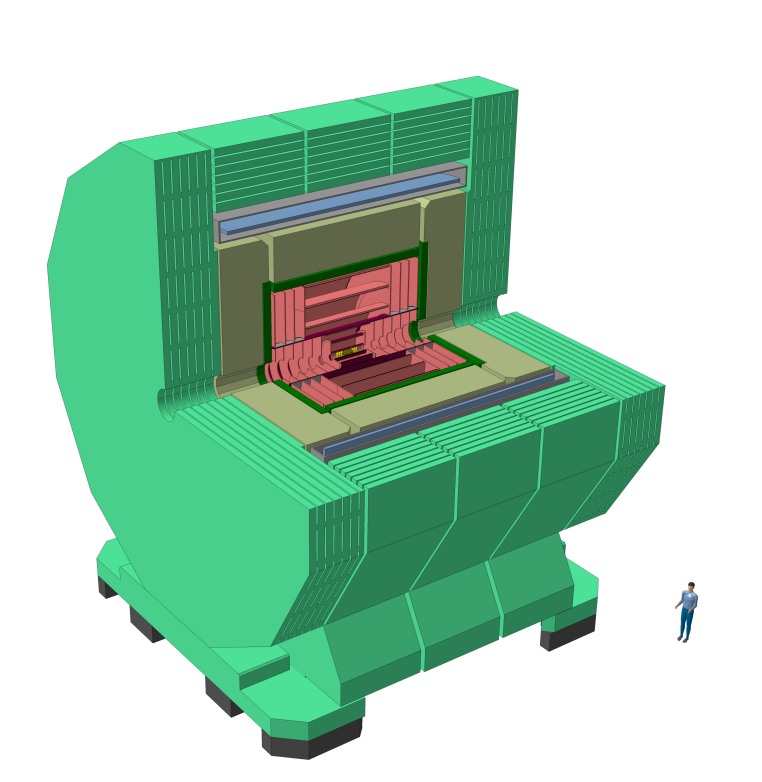
\includegraphics[width = 6.5cm, height = 5.5cm]{fcc_det/ph1.png}
    \caption{Isometric view of the CLD detector, with one quarter removed.}
    \label{fig:detector1}
\end{figure}

\begin{figure}
    \centering
    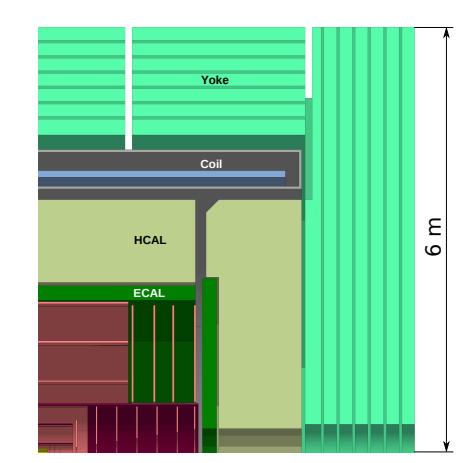
\includegraphics[width = 9cm, height = 9cm]{fcc_det/ph2.png}
    \caption{Vertical cross section showing the top right quadrant of CLD.}\label{fig:detector2}
\end{figure}

\begin{figure}
    \centering
    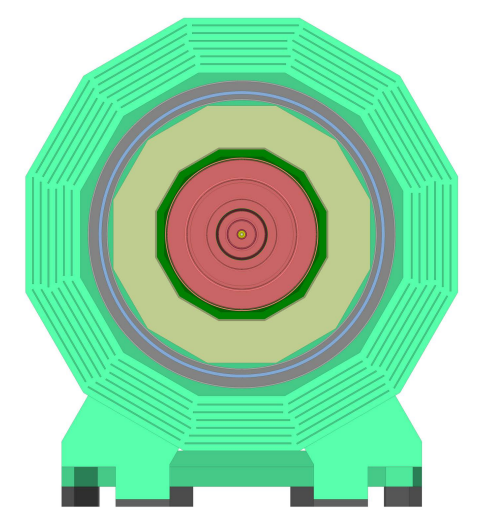
\includegraphics[width = 8cm, height = 9cm]{fcc_det/ph3.png}
    \caption{Transverse $(XY)$ cross section of CLD.}
    \label{fig:mymodel3}
\end{figure}

\section{Vertex detector}
The vertex detector in the CLD concept, a higher  version of the 
one in CLICdet, consists of a cylindrical
barrel detector closed off in the forward directions by discs. 
The layout is based on double layers, i.e.
two sensitive layers fixed on a common support structure (which 
includes cooling circuits). The barrel
consists of three double layers, the forward region is covered 
by three sets of double-discs on both sides
of the barrel. An overview of the vertex detector layout is 
given in Figure(\ref{fig:vertex}). The total area of the vertex
detector sensors is 0.53$m^2$.
\begin{figure}[ht]
    \centering
    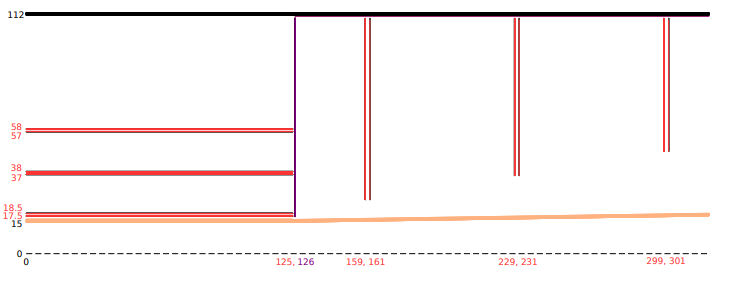
\includegraphics[width = 1\linewidth]{fcc_det/ph14.png}
    \caption{Vertex detector layout in ZR plane. Red lines indicating sensors, black lines indicating support structure and vaccume pipe in orange color.}
    \label{fig:vertex}
\end{figure}


The vertex detector consists of 
$25\times25\mu$m$^2$ pixels 
having  a silicon sensor thickness of $50\mu$m. Using
pulse height information and charge sharing, a single point 
resolution of $3\mu$m is aimed for.
The overall length of the barrel vertex detector, built from staves, is 250 mm. The double layer
structure is shown in Figure(\ref{fig:vertex2}).
The vertex detector forward region consists of three discs on 
each side where  each disc is built as a double layer device. The 
discs are located a distance from the IP of 160, 230 and 300 
mm respectively. They are
constructed from 8 trapezoids, approximating a circle. For 
simplicity the trapezoids are not overlapping
in the simulation model. The inner radii of the forward discs 
respect the 150 mrad cone reserved for MDI elements. 
\begin{figure}
    \centering
    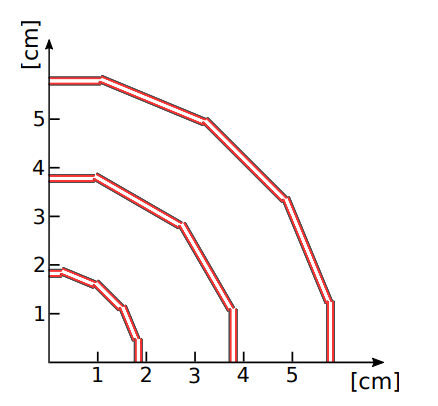
\includegraphics[width=6cm, height=6cm]{fcc_det/ph5.png}
    \caption{Vertex detector double layer structure in XY plane.}
    \label{fig:vertex2}
\end{figure}

\section{Silicon tracker}
Like  CLIC detector, the CLD concept have  an all-silicon tracker. 
The inner tracker consists of three barrel layers and seven forward discs. The outer tracker
has  an additional three barrel layers and four discs. The overall layout of the silicon tracker in CLD is shown in Figure(\ref{fig:tracking}) .
\begin{figure}[ht]
    \centering
    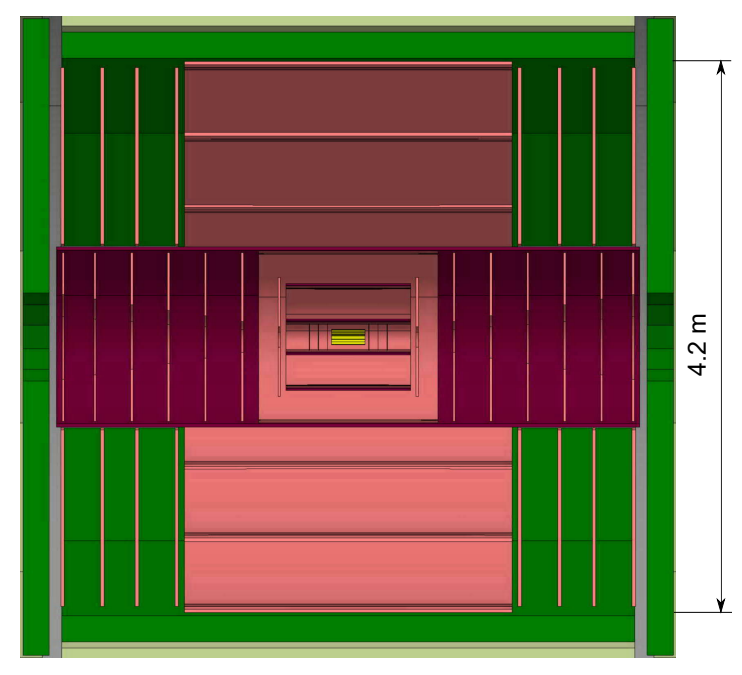
\includegraphics[width = 7cm, height = 7cm]{fcc_det/ph6.png}
    \caption{ Overall layout of the CLD tracking system: the vertex barrel detector is shown in yellow, the
    tracking layers in lighter red.  The surrounding ECAL is shown in green.}
    \label{fig:tracking}
\end{figure}
The tracking volume has a half-length of 2.2m and a maximum radius of 2.1m. This radius allows to
achieve a similar momentum resolution in the CLD tracking system with a 2T magnetic field as in the CLIC detector  tracker with a 4T field and a radius of 1.5 m. The main support tube has an inner and outer radius of 0.686m and 0.690m respectively, and a half-length of 2.3 m.
The
tracking system covers polar angles larger than 150 mrad.
The pixel vertex detector and the silicon tracker are treated as one unified tracking system in simulation and reconstruction.

\section{Electromagnetic calorimeter(ECAL)}
Further studies about  ILC and CLIC have revealed 
that high granularity particle flow calorimetry appears to be a 
promising option to reach the required jet energy resolution of 
3-4$\%$. Such a performance is necessary to allow the 
distinction e.g. of $W$ and $Z$ bosons on an event-by-event basis.
\begin{figure}[ht]
    \centering
    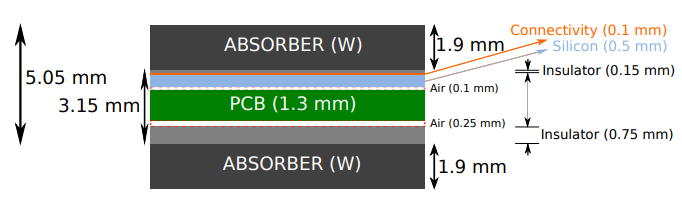
\includegraphics[width = 12cm, height = 3.5cm]{fcc_det/ph10.png}
    \caption{Schematic drawing of the ECAL segmentation as implemented in the simulation model}
    \label{fig:ecal}
\end{figure}
The segmentation of the ECAL has to be sufficient to resolve 
energy depositions from nearby particles in
high energy jets. Studies performed in the context of the ILC 
and CLIC suggest a calorimeter transverse
segmentation of $5 \times 5$mm$^2$.
The technology chosen as baseline option for the detectors at 
the linear colliders is a silicon-tungsten sandwich structure as shown in Figure(\ref{fig:ecal}).
This detector design is also implemented in the CLD simulation
model.


\section{Hadron calorimeter(HCAL)}
The  hadronic
calorimeter of CLD has a structure and granularity as the one 
in CLICdet. It consists of steel absorber
plates, each of them 19mm thick interleaved with scintillator 
tiles. The gap for the 
sensitive layers and their cassette is 7.5mm.
The polystyrene scintillator in the cassette is 3 mm thick with 
a tile size of $30 \times 30$ mm$^2$.
In the simulations,
the part of the HCAL endcap which surrounds the ECAL endcap  is 
treated as a separate
entity called the "HCAL ring". The detailed HCAL layer stack as implemented in the simulation 
model is shown in Figure(\ref{fig:hcal}).
\begin{figure}[ht]
    \centering
    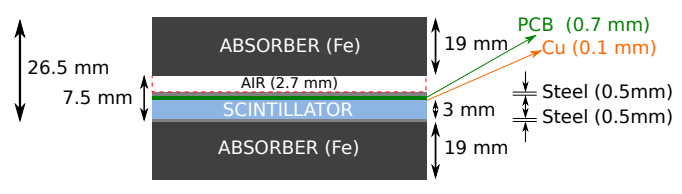
\includegraphics[width = 12cm, height = 3.5cm]{fcc_det/ph11.png}
    \caption{ Schematic drawing of HCAL segmentation as implemented in the simulation model.
    }
    \label{fig:hcal}
\end{figure}


\section{Magnet system}
The solenoid magnetic field of the CLD detector  is 2T, 
which is limited by MDI constraints. 
In the simulation model, the magnetic field in CLD is 2T 
throughout the volume inside the superconducting coil. The 
field in the yoke barrel is 1T, pointing in the opposite 
direction with respect to the
inner field. The simulation model currently assumes no field in 
the yoke endcap nor outside the yoke.


\section{Muon system}
The iron  yoke is divided  into three rings in the barrel region and the two endcaps, as shown in
Figure(\ref{fig:muon}). The thickness of the yoke is reduced w.r.t. CLICdet, in correspondence to the lower solenoid
field . A muon identification system with 6 layers as in CLICdet is implemented. An additional 7th layer
is inserted in the barrel as close as possible to the coil. This layer may serve as tail catcher for hadron
showers. The muon system layout in CLD is shown in Figure(\ref{fig:yoke}).

\begin{figure}[ht]
    \centering
    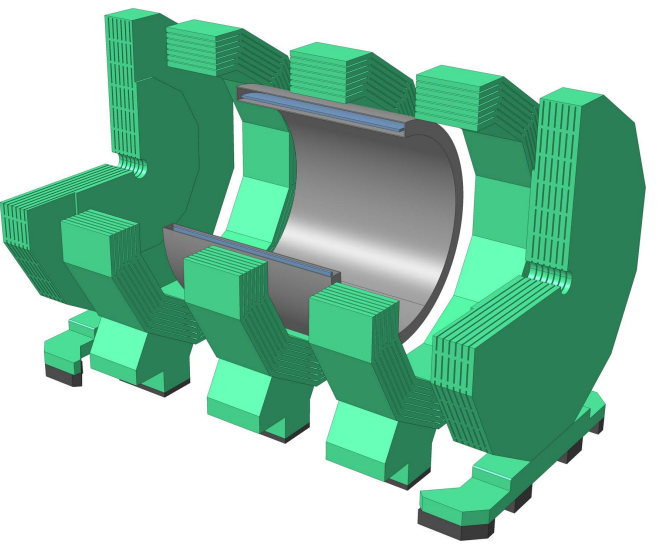
\includegraphics[width=8cm, height=6cm]{fcc_det/ph12.png}
    \caption{Segmentation of the iron return yoke of CLD into endcaps and three barrel rings.}
    \label{fig:muon}
\end{figure}

\begin{figure}[ht]
    \centering
    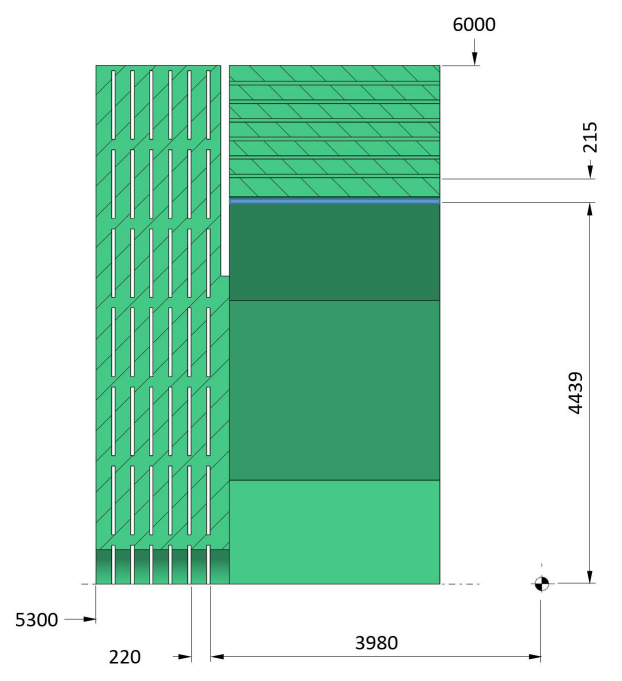
\includegraphics[width = 7cm, height = 7cm]{fcc_det/ph13.png}
    \caption{ Schematic cross section of the muon system layout in the yoke of CLD.}
    \label{fig:yoke}
\end{figure}